\documentclass[11 pt]{article}
\usepackage[utf8]{inputenc}
\usepackage[english, russian]{babel}
\usepackage[a4paper,top=1.8cm,bottom=2cm,left=2cm,right=2cm,marginparwidth=1cm]{geometry}
\usepackage{amsmath}
\usepackage{mathtools}
\usepackage{xcolor}
\usepackage{subfigure}
\usepackage{hyperref}
\usepackage{graphicx}
\usepackage{subcaption}
\usepackage{wrapfig}
\usepackage{float}


\setlength{\parindent}{0em}
\usepackage{multirow}

\begin{document}

    \begin{flushright}
    {\Large Волкова Александра, Б02-927}
    \end{flushright}
    \hrulefill
    \linespread{1.2}

    \subsection*{16. Электронные нелинейности, резонансное взаимодействие. Полуклассическая модель. Балансные уравнения. Понятие об интенсивности просветления среды. Задача о просветлении среды и изменении показателя преломления.}

    \href{ https://docs.google.com/presentation/d/16hv_WdqqJShSlDdzsJv6v4AtQ_hLnpfM/edit#slide=id.p1}{Презентация 10}



    Полуклассическое описание резонансной нелинейности:
    излучение – классическое, атом – квантовый.

    Рассматриваем двухуровневую систему, решаем уравнение Шредингера.

    Поляризация $    P = \frac{1}{2} (B e^{-i \omega t } + C) $

    \begin{align}
        \frac{d B}{d t} = i \frac{d^2}{\hbar}(N_1 - N_2) - i (\omega_0 - \omega) - \frac{B}{T_2} \\
        \frac{d N_2}{d t} = - \frac{i}{4 \hbar} (BA^* - B^*A) - \frac{N_2}{T_1}
    \end{align}

    Искусственно добавляем времена продольной и поперечной релаксации $T_1$ и $T_2$.

    Стационарное решение $\frac{d B}{d t} = 0$ даёт коэффициенты преломления и поглощения

    \begin{figure}[h]
        \centering
        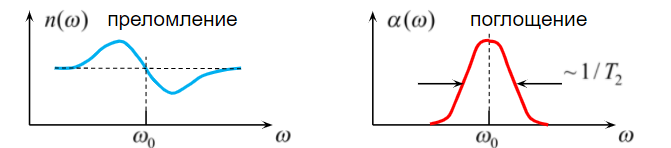
\includegraphics[width=0.6\textwidth]{16-1.png}
        \label{fig:my_label}
    \end{figure}


    В зависимости от длительности светового импульса возможны режимы

    \begin{figure}[h]
        \centering
        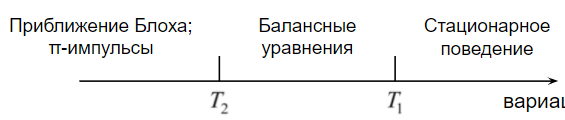
\includegraphics[width=0.5\textwidth]{16-2.png}
        \label{fig:my_label}
    \end{figure}

    Балансные уравнения дают сечение поглощения $\sigma(\omega)$ и

    \begin{align}
        \frac{d I}{d t} = \sigma (N_2 - N_1) I \\
        \frac{d N_2}{d t } = \sigma (N_1 - N_2) \frac{I}{\hbar \omega} - \frac{N_2}{T_1}
    \end{align}

    В стационарном режиме $\frac{d N_2}{d t } = 0$ возникает величина интенсивности насыщения $I_{sat}$ и

    \begin{equation}
        \frac{d I }{d t} = - \frac{\sigma N}{1 + \frac{I}{I_{sat}}} I
    \end{equation}

    Эффект просветления -- увеличение прозрачности при возрастании интенсивности падающего света

    \subsection*{17. Методы измерения констант нелинейного взаимодействия: метод z-сканирования.}

    \href{https://docs.google.com/presentation/d/1EXS66mVOTrJ9DTWXtli-Kh3TE5-qSYC4/edit#slide=id.p20}{Презентация 8} один слайд

    Метод измерения нелинейного показателя преломления, использующий эффект самофокусировки.

    Измеряется зависимость энергии лазерного излучения, прошедшего через диафрагму, то есть коэффициент пропускания, в зависимости от положения образца относительно фокуса линзы. Затем из этой зависимости можно получить $n_2$ и Re$\chi^{(3)}$.

    Для измерения мнимой части $\chi^{(3)}$ диафрагму убирают и измеряют коэффиент поглощения.

    \subsection*{18. «Ядерные» нелинейности. Роль стрикционного и ориентационного механизмов нелинейности.}

    \href{https://docs.google.com/presentation/d/1K_ZGFk-pBl2Iq715U5IDb6fHsFmTuww9/edit#slide=id.p16}{Презентация 6.14.10.21} последние слайды

    \begin{itemize}
        \item Стрикционная нелинейность

        Втягивание вещества в область повышенного поля (втягивание диэлектрической жидкости в конденсатор). Наблюдается во всех средах

        \item Ориентационная нелинейность. Поворот анизотропных молекул вдоль электрического поля волны, наблюдается в жидкостях и газах

        \item тепловая нелинейность

        \item плазменная нелинейность

    \end{itemize}

    Стрикционная и ориентационная нелинейности возникают с запаздыванием, у них есть характерные времена релаксации, значительно превышающие период световой волны.

    Ядерные нелинейности вызывают кубичные нелинейные явления $\chi^{(3)}$.

    \subsection*{19. Вынужденное комбинационное рассеяние (ВКР). Роль спонтанного рассеяния. Основные характеристики излучения ВКР. Особенности энергообмена между волнами при ВКР.}

    \href{https://docs.google.com/presentation/d/1AFszmR3vaV3yd9CE1-JN2BAv94PDQvBh/edit#slide=id.p3}{Презентация 11.02.12.21}

    ВКР вызвано колебаниями молекул, то есть переменной поляризуемостью среды.

    Возникают две новые линии излучения, отстоящие по частоте от основной на $\hbar \omega = E_{\text{кол}}$

    Интенсивность не зависит от угла рассеяния, зависит от температуры.

    \begin{equation}
        \frac{I_{\text{стокс}}}{I_{\text{антистокс}}} \gg \exp(-\frac{\hbar \omega}{k T})
    \end{equation}

    Основная и рассеянная волны складываются, итоговая интенсивность осциллирует на частоте молекулярных колебаний, что поддерживает возбуждение новых колебаний.

    \begin{figure}[h]
        \centering
        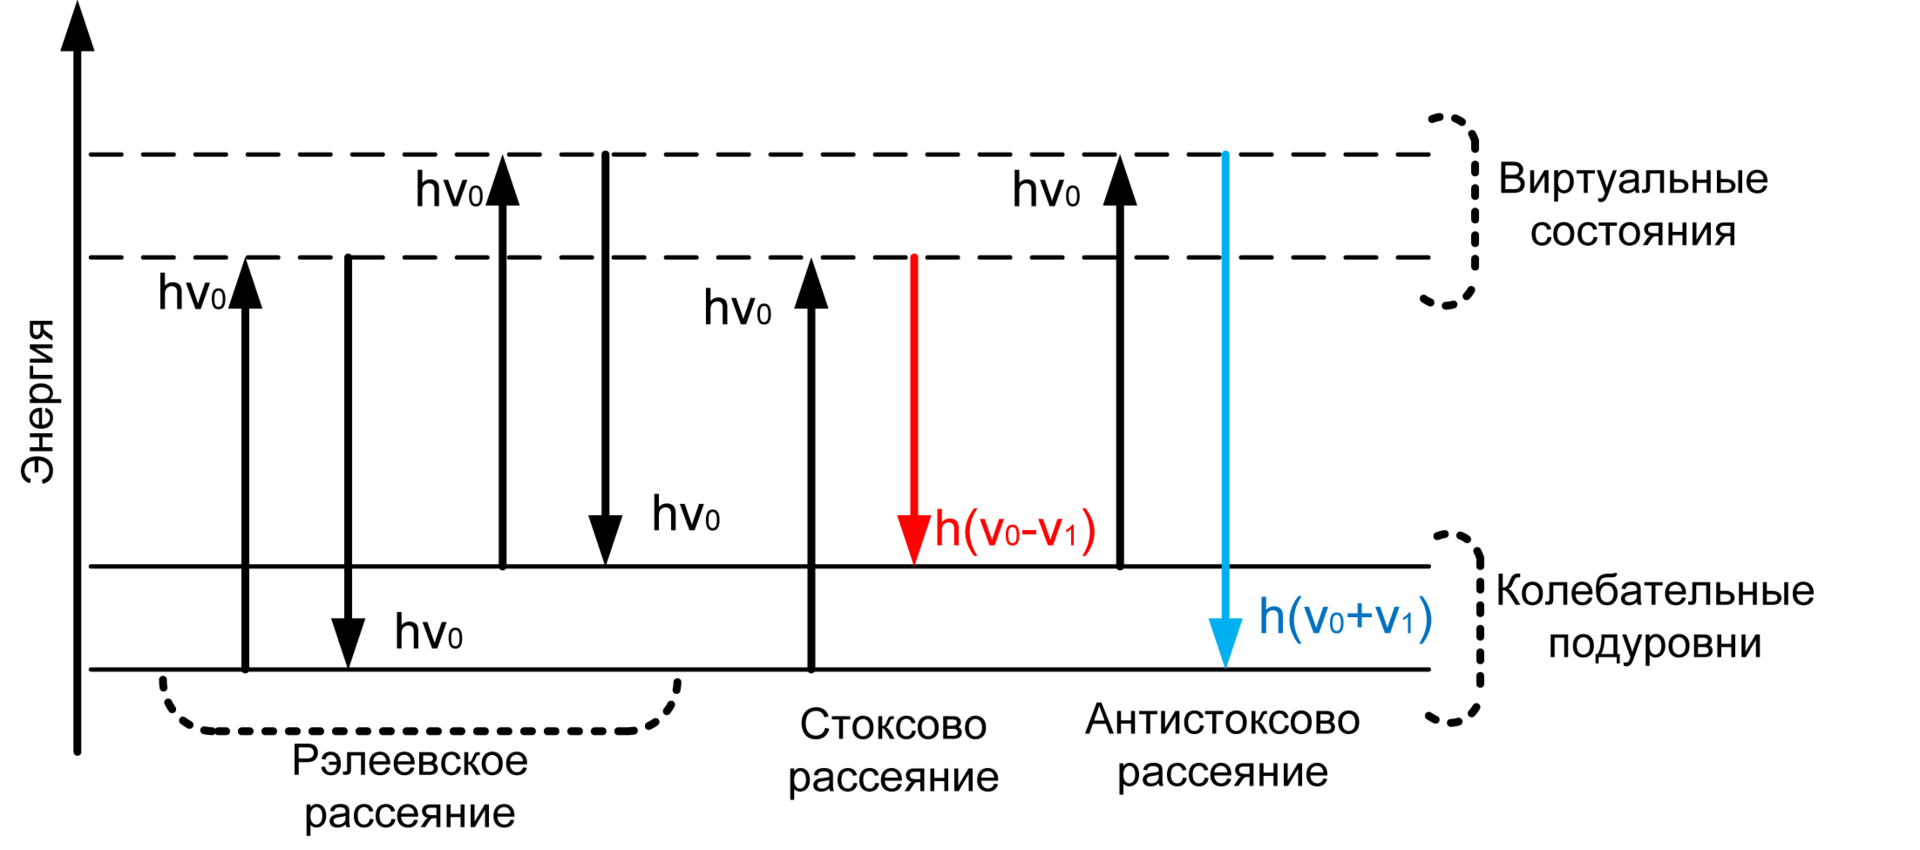
\includegraphics[width=0.6\textwidth]{19-1.png}
        \label{fig:my_label}
    \end{figure}

    Способ описания -- система с двумя уровнями энергии, для которой решается уравнение Шредингера.

    Волна на стоксовой частоте усиливается, на антистоксовой ослабевает.

    \subsection*{20. Вынужденное рассеяние Мандельштама-Бриллюена (ВРМБ). Роль спонтанного рассеяния. Основные характеристики излучения ВРМБ. Особенности энергообмена между волнами при ВРМБ.}

    \href{https://docs.google.com/presentation/d/1c5RS2UDGEx-meePbZZv-neXMGNQ4FEft/edit#slide=id.p2}{Презентация 12.09.12.21}

    Звуковые волны в среде создают периодические неоднородности плотности, которые можно считать
    объёмными дифракционными решетками.

    ВРМБ вызвано дифракцией световых волн на таких неоднородностях среды.

    Условия дифракции Брегга:
    \begin{enumerate}
        \item фронты звуковых волн служат отражающими поверхностями для световых волн
        \item $\Lambda \sin \frac{\Theta}{2} = \lambda$, где $\Lambda$ -- длина звуковой волны
    \end{enumerate}

    ВРМБ -- кубичная нелинейность.

    Смешение по частоте рассеянных волн зависит от угла и максимально для обратного рассеяния $\Delta \nu = \frac{2 v_{\text{зв}}}{\lambda}$.

    Основная и рассеянная волны складываются, итоговая интенсивность осциллирует на частоте звуковой волны, что поддерживает возбуждение новых колебаний среды.

    Способ описания -- система с двумя уровнями энергии, для которой решается уравнение Шредингера.

    Волна на стоксовой частоте усиливается, на антистоксовой ослабевает.

\end{document}